\documentclass[aspectratio=169, table]{beamer}


%\usepackage[beamertheme=./praditatheme]{Pradita}

\usetheme{Pradita}

\title{Chapter-03: Model-View-Controller (MVC) Architecture}
\subtitle{IF231303-Software Architecture\\Pradita University}
\author{Alfa Yohannis}
\begin{document}
	
	\begin{frame}[plain]
		\maketitle
	\end{frame}
	
	\begin{frame}{Model-View-Controller Schema}
		\begin{figure}[h]
			\centering
			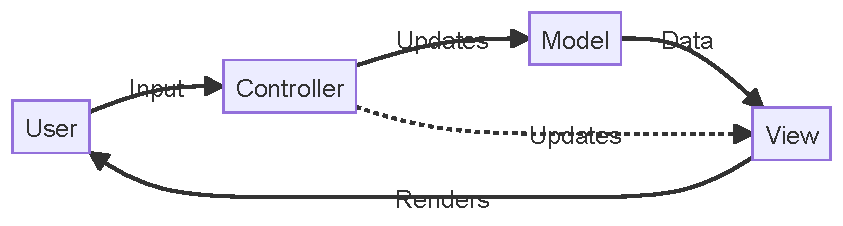
\includegraphics[width=\textwidth]{mvc}
			\caption{Model-view-controller (MVC) architecture.}
			\label{fig:mvc}
		\end{figure}
	\end{frame}
	
	\begin{frame}{Background}
		\begin{itemize}
			\item In the beginning, software development put the functions of graphical user interface (GUI) and data management into one code, with no separation of concerns.
			\item Model-view-controller (MVC) was proposed to solve the problem of users controlling a large and complex data set.
		\end{itemize}
	\end{frame}
	
	\begin{frame}{Model-view-controller (MVC)}
		\begin{itemize}
			\item One of the architectural patterns for developing Graphical User Interface (GUI).
			\item It divides program logic into three interconnected components: Model, View, and Controller.
			\item \textbf{Model} manages the data, logic, and rules of the application.
			\item \textbf{View} is the presentation that users can see and interact with, e.g., webpages, desktop GUI, charts, buttons, text fields, etc.
			\item \textbf{Controller} accepts user inputs via the view and pass them to the model to be handled. It also retrieves data from the model to be displayed on the view so that users can see.
			
		\end{itemize}
	\end{frame}
	
	\begin{frame}{Advantages}
		MVC brings higher modularity (lower coupling) through separation of concerns:
		\begin{itemize}
			\item The separation of presentation and data allows model can have multiple views simultaneously.
			\item Composable presentation. A view can have one or more sub-views.
			\item Switchable input modes. A controller can replace another controller at runtime.
			\item Different mechanisms of input and output processing via the separate responsibilities of controllers and views.
			\item Data engineers, backend and frontend developers can focus on their main tasks, e.g., managing data, coding business logics and interface respectively.
		\end{itemize}
	\end{frame}
	
	\begin{frame}{Disadvantages}
		\begin{itemize}
			\item Introduce certain degree of complexity since code has to be divided into three different abstractions.
			\item Developers need to follow certain strict rules in defining controllers, models, views.
			\item Relatively hard to understand due to its structure.
			\item It can be overkill for small projects.
			\item It's best for UI development but might not the best for other types of developments and  applications.
			\item The different, layered abstractions slow down performance.
		\end{itemize}
	\end{frame}
	
	\begin{frame}{Other MVC Variants}
		\begin{itemize}
			\item Model-View-Presenter (MVP).
			\item Model-View-ViewModel (MVVM).
			\item Model-View-Adapter (MVA).
			\item Hierarchical Model-View-Controller (HMVC).
			
		\end{itemize}
	\end{frame}
	
\end{document}
